% =============================================================================
% FIRE 2026 — Regular Paper (DOUBLE-BLIND)
% ACM ICPS, sigconf, two columns. Maximum 9 pages of content, references excluded.
%
% Anonymity: no author names, no affiliation, no repository URL that identifies
% the authors. Concrete links are restored in the camera-ready.
% =============================================================================
\documentclass[sigconf,natbib=true,anonymous=true]{acmart}

\AtBeginDocument{%
  \providecommand\BibTeX{{\normalfont B\kern-0.5em{\scshape i\kern-0.25em b}\kern-0.8em\TeX}}}

\setcopyright{none}
\settopmatter{printacmref=false}
\renewcommand\footnotetextcopyrightpermission[1]{}
\pagestyle{plain}
\acmConference[FIRE 2026]{Forum for Information Retrieval Evaluation}{December
  2026}{India}

\usepackage{booktabs}
\usepackage{adjustbox}
\usepackage{graphicx}
\usepackage{amsmath}

\begin{document}

\title{Does Weight Sharing Reduce Stereotype Association? An Iso-Loss
       Comparison of Looped Transformer Encoders}

\author{Anonymous Author(s)}

% ------------------------------------------------------------------- abstract
\begin{abstract}
A pre-trained encoder is built once and then reused, so any stereotypical
association it holds is passed on to every system that adopts it. Encoders that
apply one block of weights at several depths, known as looped or recursive
models, are attractive because they keep effective depth at a lower storage cost.
Whether such reuse also changes what a model records about social groups is not
known, and the question is awkward to answer: a shared model and an unshared
model of the same size do not reach the same language modelling quality, and a
better trained model gives sharper answers on every probe. This study compares
four encoders at matched validation loss rather than at matched parameters or
matched tokens, so that a difference in measured association cannot be explained
by one model having learned more language. On a paired stereotype benchmark of
1508 items, the two weight-shared encoders record a lower stereotype effect size
than the unshared baseline, and both contrasts survive correction for multiple
comparisons. Adding parallel streams and hyper-connections on top of looping
gives no further reduction and makes training less stable. The same models answer
at chance on a coreference instrument, so the result is reported as a statement
about association in the masked language modelling head at this training scale,
and not as evidence about downstream behaviour.
\end{abstract}

% ---------------------------------------------------------- CCS and keywords
\begin{CCSXML}
<ccs2012>
<concept>
<concept_id>10010147.10010178.10010179</concept_id>
<concept_desc>Computing methodologies~Natural language processing</concept_desc>
<concept_significance>500</concept_significance>
</concept>
<concept>
<concept_id>10010147.10010257.10010258</concept_id>
<concept_desc>Computing methodologies~Learning paradigms</concept_desc>
<concept_significance>300</concept_significance>
</concept>
<concept>
<concept_id>10003456.10010927</concept_id>
<concept_desc>Social and professional topics~User characteristics</concept_desc>
<concept_significance>300</concept_significance>
</concept>
</ccs2012>
\end{CCSXML}

\ccsdesc[500]{Computing methodologies~Natural language processing}
\ccsdesc[300]{Computing methodologies~Learning paradigms}
\ccsdesc[300]{Social and professional topics~User characteristics}

\keywords{social bias, masked language models, parameter sharing, looped
transformers, fairness evaluation, iso-loss comparison}

\maketitle

% =============================================================== introduction
\section{Introduction}

Pre-trained encoders sit underneath much of current retrieval and text
classification practice. One masked language model is trained and then reused
across many tasks, so a stereotypical association acquired during pre-training is
inherited by every system built on top of it. Which design choices change these
associations is therefore a question about shared infrastructure rather than
about a single application.

Weight sharing across depth is one such choice. ALBERT ties a single transformer
block across all layers and reaches competitive quality at a fraction of the
storage \citep{lan2020albert}. Recent work applies a small block repeatedly to
obtain effective depth without a matching parameter count, and reports gains on
reasoning tasks \citep{saunshi2025looped,bae2025mor}. The motivation offered for
these designs is efficiency. A separate line of work finds that changing model
capacity changes what a model records about social groups: pruning and
quantisation shift error rates unevenly across demographic groups
\citep{hooker2020characterising,xu2022compression,ramesh2023comparative}. Read
together, these two lines raise a question that neither answers. If a looped
encoder must cover twelve depths of computation with six blocks of weights, does
the pressure to reuse those blocks suppress the narrow item-level associations
that stereotype benchmarks detect?

A confound stands in the way of an answer. A shared encoder and an unshared
encoder with the same parameter count do not reach the same language modelling
quality. A model further along in training also gives sharper predictions on
every probe, stereotype probes included. Comparing two architectures after a
fixed number of training tokens therefore measures training progress together
with architecture. Existing comparisons of compression and
fairness do not control for this directly, which makes their results hard to
attribute to one cause.

This work removes the confound by matching on outcome rather than on budget. Each
encoder is trained until its validation loss crosses a list of values fixed in
advance, and a snapshot is written at each crossing. Encoders are then compared
only at snapshots of equal validation loss. Under this protocol a difference in
measured association cannot be explained by one model having learned more of the
language.

Four encoders are compared: an unshared baseline; a looped encoder that applies
six blocks twice; an ALBERT-style encoder that applies one block twelve times;
and a looped encoder extended with four parallel residual streams joined by
hyper-connections \citep{zhu2025hyperconnections}. The last of these tests whether
routing capacity added on top of sharing changes the picture.

This paper makes three contributions.

\begin{enumerate}
\item An iso-loss protocol that attributes a difference in measured stereotype
      association to architecture rather than to training progress, together with
      a capability gate that states when the measurement is interpretable.
\item A controlled comparison of four encoders under this protocol, in which both
      weight-shared encoders record a lower stereotype effect size than the
      unshared baseline at matched validation loss.
\item A negative result: parallel streams and hyper-connections added on top of
      looping give no further reduction, and make optimisation less stable.
\end{enumerate}

Section~\ref{sec:related} reviews prior work on bias measurement and on weight
sharing. Section~\ref{sec:method} defines the encoders, the matching protocol and
the measures. Section~\ref{sec:setup} gives the training setup and
Section~\ref{sec:results} reports results. Section~\ref{sec:limits} states what
the evidence does not support.

% ================================================================ related work
\section{Related Work}
\label{sec:related}

\paragraph{Measuring stereotype association in masked models.}
CrowS-Pairs scores a model on minimal pairs that differ only in a demographic
term and records how often the stereotypical member receives the higher
pseudo-log-likelihood \citep{nangia2020crows}. StereoSet uses a related paired
construction with an added language modelling score \citep{nadeem2021stereoset}.
\citet{kurita2019measuring} introduced the masked-position probing that both
build on. The instruments have known weaknesses. \citet{blodgett2021salmon}
audited these benchmarks and found unclear or inconsistent items in a large share
of pairs, and warned against reading one aggregate number as a measure of harm.
\citet{wang2025difference} separate correlation-type benchmarks, which record
association, from descriptive and normative benchmarks, which record whether a
model treats groups differently when it should. The measure used here is of the
correlation type, and Section~\ref{sec:limits} states what follows from that.

\paragraph{Weight sharing and looped depth.}
ALBERT ties one encoder block across all layers and trades quality for storage
\citep{lan2020albert}. \citet{saunshi2025looped} show that a $k$-layer block
looped $L$ times approaches the reasoning performance of a $kL$-layer model, and
argue that depth rather than parameter count drives several reasoning tasks.
\citet{bae2025mor} learn a per-token recursion depth over a shared block.
\citet{geiping2025huginn} scale a recurrent-depth model to test-time compute, and
\citet{zhu2025ouro} and \citet{frey2026adaptive} study related looped language
models. Hyper-connections generalise the residual connection to several parallel
streams with learned mixing \citep{zhu2025hyperconnections}, later constrained to
a manifold by \citet{xie2025mhc}, and \citet{zeitoun2026hyperloop} combine looping
with hyper-connections. This body of work evaluates quality, efficiency and
reasoning. It does not report the effect of sharing on social bias.

\paragraph{Capacity, compression and fairness.}
\citet{hooker2020characterising} found that pruning degrades accuracy unevenly
across groups, with a small subset of examples absorbing most of the damage.
\citet{xu2022compression} and \citet{ramesh2023comparative} report mixed outcomes
for compression and fairness in language models, with the direction depending on
the compression method and the benchmark. \citet{voria2026tracing} localise
stereotype-carrying neurons inside pre-trained transformers. These studies
compress a model after training. The present work varies sharing before training
and compares at matched quality, which separates the architectural question from
the recovery dynamics of a compressed checkpoint.

% ===================================================================== method
\section{Method}
\label{sec:method}

\subsection{Architectures}

All four encoders use hidden size 768, twelve effective depths, one tokeniser and
the same masked language modelling objective \citep{devlin2019bert}. They differ
only in how weights are reused across depth.

\emph{VanillaBERT} holds twelve independent blocks and is the unshared control.
\emph{LoopedBERT} holds six blocks and applies the stack twice, halving the
depth-unique parameters. \emph{ALBERTLoopedBERT} holds one block and applies it
twelve times, the extreme point of the sharing axis \citep{lan2020albert}.
\emph{HyperloopBERT} keeps the six-block loop and adds four parallel residual
streams joined by hyper-connections \citep{zhu2025hyperconnections}. Instead of a
single residual path, the model carries $n$ streams and mixes them at each depth
with a learned matrix,
%
\begin{equation}
\mathbf{H}^{(\ell+1)} = \mathbf{A}^{(\ell)}\mathbf{H}^{(\ell)}
                      + \mathbf{B}^{(\ell)} f\!\left(\mathbf{H}^{(\ell)}\right),
\end{equation}
%
where $\mathbf{H}^{(\ell)} \in \mathbb{R}^{n \times d}$ stacks the $n$ stream
states of width $d$ at depth $\ell$, $f$ is the shared transformer block,
$\mathbf{A}^{(\ell)} \in \mathbb{R}^{n \times n}$ is a learned matrix that mixes
the streams, and $\mathbf{B}^{(\ell)} \in \mathbb{R}^{n \times n}$ distributes the
block output back across them. Setting $n = 1$ with
$\mathbf{A} = \mathbf{B} = 1$ recovers the ordinary residual connection.
Table~\ref{tab:arch} gives the resulting sizes.

\begin{table}[t]
\centering
\caption{The four encoders. All use hidden size 768 and twelve effective depths,
and differ only in weight reuse across depth.}
\label{tab:arch}
\small
\begin{adjustbox}{max width=\columnwidth}
\begin{tabular}{lccc}
\toprule
Architecture & Unique blocks & Parameters & Shared ratio \\
\midrule
VanillaBERT       & 12 & 110.1\,M & 0.00 \\
LoopedBERT        &  6 &  67.6\,M & 0.50 \\
HyperloopBERT     &  6 &  86.5\,M & 0.50 \\
ALBERTLoopedBERT  &  1 &  32.1\,M & 0.92 \\
\bottomrule
\end{tabular}
\end{adjustbox}
\end{table}

\subsection{Iso-loss matching}

The comparison is defined on outcome rather than on budget. A list of target
validation loss values is fixed before training. Validation loss is measured at a
regular interval during a run, and the first time it falls below a target the
model state is written to disk as the snapshot for that band. Encoders are then
compared only at snapshots that carry the same band.

Two properties of the protocol affect how the results are read. Several bands are
sometimes crossed inside one validation interval, in which case they share a
single snapshot; the analysis therefore treats a distinct validation loss, not a
band label, as the unit of measurement. Matching is also approximate, since a
snapshot is taken at the first measurement below the target and the realised loss
sits a little below the nominal value. The realised spread at the comparison point
is reported in Section~\ref{sec:results}.

\subsection{Stereotype measure}

Each benchmark item is a pair of sentences differing only in a demographic term,
one member marked stereotypical and the other anti-stereotypical
\citep{nangia2020crows}. For a sentence $s$ with tokens $t_1 \dots t_T$, the
pseudo-log-likelihood masks one position at a time and sums the resulting log
probabilities,
%
\begin{equation}
\mathrm{PLL}(s) = \sum_{i=1}^{T} \log P\!\left(t_i \mid s_{\setminus i}\right),
\end{equation}
%
where $s_{\setminus i}$ is the sentence with position $i$ replaced by the mask
token and $P$ is the output of the masked language modelling head. Scoring runs in
32-bit precision, because reduced precision reorders closely matched pairs.

For a pair, the effect size is the length-normalised difference
$\left(\mathrm{PLL}(s_{\text{stereo}}) - \mathrm{PLL}(s_{\text{anti}})\right)/T$,
and the reported statistic is its mean over items with a bootstrap confidence
interval. Zero means the model has no preference between the two members.
Encoders are contrasted item by item, so each pair contributes one paired
difference and the test is a paired permutation test, corrected across the three
contrasts by the Holm procedure. Permutation $p$-values follow
\citet{phipson2010permutation}, which avoids reporting an exact zero.

\subsection{Capability gate}
\label{sec:gate}

A model that predicts almost nothing returns near-tied pseudo-log-likelihoods and
so a small effect size, which would be indistinguishable from a genuinely
unbiased model. The protocol therefore fixes in advance three conditions under
which a bias reading is treated as interpretable. The model must score above
chance on a set of GLUE tasks \citep{wang2018glue}. The effect-size interval of
the unshared baseline must exclude zero. The model must also score above chance on
the pro-stereotype split of a coreference instrument \citep{zhao2018winobias},
which tests whether it can resolve the pronoun at all.
Section~\ref{sec:capability} reports the outcome of this gate, which governs how
the main result should be read.

% ====================================================================== setup
\section{Experimental Setup}
\label{sec:setup}

All four encoders are pre-trained on the same 7 billion tokens of FineWeb-Edu
\citep{penedo2024fineweb} at sequence length 128, with a tokeniser fitted once and
reused, so no encoder sees a different corpus or segmentation. The corpus is
pre-tokenised into fixed-size blocks and stored as a memory-mapped array, and an
integrity check compares the tokeniser checksum and block count against a manifest
at the start of every run. Training uses AdamW at a peak learning rate of
$3 \times 10^{-4}$, batch size 512, warmup over a tenth of the steps, gradient
clipping at 1.0, and bfloat16 autocast with FlashAttention
\citep{dao2022flashattention}. Runs execute on one H100 GPU.

HyperloopBERT is the single exception to the shared learning rate. At
$3 \times 10^{-4}$ it diverged to a non-finite loss, and at half that value it
diverged later in training; Section~\ref{sec:stability} reports both events. Its
released snapshots come from the run at $1.5 \times 10^{-4}$. Holding the learning
rate fixed across all four would have compared three stable models against one
broken configuration. The peak learning rate is therefore tuned per architecture,
and the arms are matched on validation loss rather than on hyper-parameters.

Results come from one seed. This constrains the strength of the claims and is
taken up in Section~\ref{sec:limits}.

% ==================================================================== results
\section{Results}
\label{sec:results}

\subsection{Language modelling quality}

Quality falls as weight reuse rises, and the cost is far from linear. Halving the
depth-unique blocks from twelve to six costs little, whereas collapsing six blocks
to one costs several times more. Figure~\ref{fig:training} shows the trajectories.
VanillaBERT and LoopedBERT lie on top of each other for most of training and
separate only slightly at the end, while ALBERTLoopedBERT stays clearly above
both. LoopedBERT is therefore not under real capacity pressure at this scale;
ALBERTLoopedBERT is.

Figure~\ref{fig:training} also shows a property the tables cannot. HyperloopBERT
leaves the early plateau, where a masked language model predicts little beyond
token frequency, after roughly half a billion tokens, while VanillaBERT and
LoopedBERT stay on it until about 1.4 billion. It reaches the comparison point
with about a quarter fewer tokens than the unshared baseline. The same run later
diverges.

\begin{figure}[t]
\centering
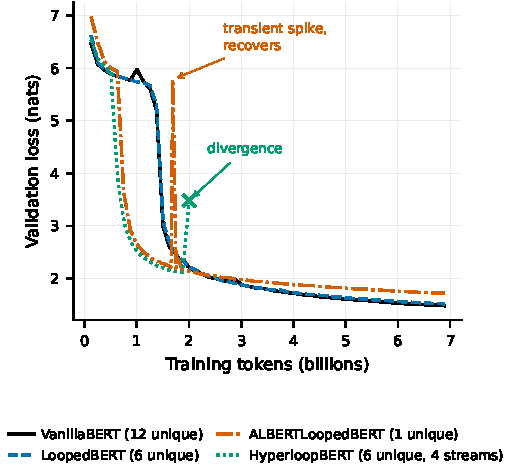
\includegraphics[width=\columnwidth]{images/fig2_training_dynamics.pdf}
\caption{Validation loss against training tokens. HyperloopBERT leaves the
plateau earliest and later diverges. ALBERTLoopedBERT shows one transient spike
that recovers.}
\label{fig:training}
\end{figure}

\subsection{Stereotype association at matched quality}

Figure~\ref{fig:isoloss} plots the stereotype effect size against realised
validation loss. Two patterns stand out. For every encoder the effect size grows
as training proceeds, so a better model records a stronger stereotype preference:
the association is acquired along with the language. At the lowest-loss end the
unshared baseline separates upward from the two shared encoders.

\begin{figure}[t]
\centering
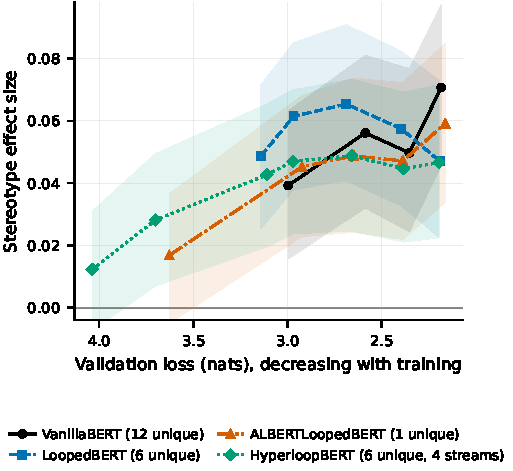
\includegraphics[width=\columnwidth]{images/fig1_isoloss_bias.pdf}
\caption{Stereotype effect size against realised validation loss with bootstrap
confidence intervals. Effect size grows as loss falls for all four encoders.}
\label{fig:isoloss}
\end{figure}

Table~\ref{tab:band} reports the comparison point. The four snapshots are matched
to within 0.034 nats, so the remaining differences cannot be attributed to one
model being better trained. LoopedBERT and HyperloopBERT record the lowest effect
sizes, VanillaBERT the highest, and ALBERTLoopedBERT sits between them.

\begin{table}[t]
\centering
\caption{Comparison point. All four snapshots lie within 0.034 nats of one
another. Effect size carries a bootstrap interval over 1508 paired items.}
\label{tab:band}
\footnotesize
\begin{adjustbox}{max width=\columnwidth}
\begin{tabular}{lccc}
\toprule
Architecture & Val.\ loss & Effect size & 95\% interval \\
\midrule
VanillaBERT       & 2.183 & 0.071 & [0.046, 0.097] \\
LoopedBERT        & 2.192 & 0.047 & [0.023, 0.073] \\
ALBERTLoopedBERT  & 2.163 & 0.059 & [0.034, 0.085] \\
HyperloopBERT     & 2.196 & 0.047 & [0.022, 0.072] \\
\bottomrule
\end{tabular}
\end{adjustbox}
\end{table}

The contrasts fixed in advance appear in Table~\ref{tab:confirm}. Both comparisons
against the unshared baseline hold after Holm correction, and the comparison
between the two shared encoders does not. Weight sharing goes with a lower
stereotype effect size at matched quality, and the extra machinery in
HyperloopBERT adds nothing beyond what plain looping already provides. The paired
effects are small, close to a tenth of a standard deviation.

\begin{table}[t]
\centering
\caption{Contrasts fixed in advance, paired permutation test over 1508 items with
Holm correction.}
\label{tab:confirm}
\footnotesize
\begin{adjustbox}{max width=\columnwidth}
\begin{tabular}{lcccc}
\toprule
Contrast & $\Delta$ & $p_{\mathrm{Holm}}$ & Cohen's $d$ & Holds \\
\midrule
Vanilla vs.\ Looped    & 0.0237 & 0.0003 & 0.115 & yes \\
Vanilla vs.\ Hyperloop & 0.0241 & 0.0004 & 0.098 & yes \\
Looped vs.\ Hyperloop  & 0.0005 & 0.4668 & 0.002 & no  \\
\bottomrule
\end{tabular}
\end{adjustbox}
\end{table}

\subsection{The capability gate is not met}
\label{sec:capability}

The gate of Section~\ref{sec:gate} is not satisfied. On the coreference
instrument all four encoders answer at chance, with pro-stereotype accuracy
between 0.489 and 0.503 and a pro-minus-anti gap within 0.03 of zero throughout. A
model that cannot resolve the pronoun cannot show a stereotypical preference in
resolving it, so this leg returns no evidence in either direction. The GLUE leg
did not yield usable numbers within the available compute and is likewise unmet.

The second leg is met: the effect-size interval of the unshared baseline excludes
zero at the comparison point, as Table~\ref{tab:band} shows. The consequence is
that the architecture contrast is a statement about pseudo-log-likelihood
association in the masked language modelling head, not a claim about behaviour on
a downstream task. Stating this openly is preferable to presenting the contrast as
a general fairness result.

\subsection{What the models predict}

Aggregate scores hide what a model actually returns, so Table~\ref{tab:qual}
reports masked-position output at the comparison point as log-odds in favour of
the masculine pronoun. Two readings follow. The occupational association is
visible directly, and it is strongest on the scientist probe for every encoder.
The secretary probe then shows why the paired design is needed: the common
stereotype runs towards the feminine pronoun, yet every encoder prefers the
masculine one, because raw pronoun frequency dominates at this scale. A single
probe would mislead, and only the paired difference isolates the demographic term.

\begin{table}[t]
\centering
\caption{Masked-position log-odds in favour of ``he'' at the comparison point. A
positive value prefers the masculine pronoun.}
\label{tab:qual}
\footnotesize
\begin{adjustbox}{max width=\columnwidth}
\begin{tabular}{lrrrr}
\toprule
Probe & Vanilla & Looped & ALBERT & Hyperloop \\
\midrule
The doctor \ldots       & $+1.47$ & $+2.33$ & $+1.30$ & $+0.46$ \\
The secretary \ldots    & $+3.00$ & $+2.60$ & $+3.80$ & $+2.71$ \\
The scientist \ldots    & $+4.22$ & $+2.76$ & $+3.65$ & $+2.93$ \\
The teacher \ldots      & $-1.76$ & $+1.04$ & $+0.26$ & $-0.29$ \\
\bottomrule
\end{tabular}
\end{adjustbox}
\end{table}

\subsection{Why the extra streams do not help}
\label{sec:mech}

The null result invites a mechanistic question: do the four streams carry
different information at all? If they collapse onto one another, the extension is
inert by construction and the null is uninformative. Two measurements address
this.

The first records how far the streams drift apart. Disagreement between streams
is near zero at the first loop depth and rises to about 0.40 by the fourth, so
the streams do separate rather than collapse. The extension is therefore active.
The second measurement relates that disagreement to bias item by item. Across
loop depths the correlation between stream disagreement and the per-item effect
size stays below 0.17 in absolute value, and none of the correlations reaches
significance at the 0.05 level. The streams differentiate, but where they
differentiate is unrelated to which items carry a stereotype preference.

For comparison, representational similarity inside LoopedBERT falls steadily with
depth distance: adjacent applications of the shared block remain close, while the
first and last differ substantially. The shared block therefore performs
different work at different depths, which is the property looped models are
designed to have. Taken with the null contrast in Table~\ref{tab:confirm}, the
reading is that the stereotype reduction observed here follows from sharing
weights across depth, and not from how information is routed once shared.

\subsection{Training stability}
\label{sec:stability}

The stream and hyper-connection extension is harder to optimise. At a peak
learning rate of $3 \times 10^{-4}$, the value that trains the other three
encoders without incident, HyperloopBERT reached a validation loss of 2.53 and
then rose to 6.86 within one interval before becoming non-finite. Halving the peak
learning rate delayed the failure rather than removing it: the model trained past
the earlier failure point, reached 2.12, and then diverged again. Both events
began shortly after the model's fastest descent.

ALBERTLoopedBERT, the most heavily shared encoder, also showed one transient loss
spike that recovered within a thousand steps, marked in
Figure~\ref{fig:training}. Together the two observations suggest that reusing
weights across depth makes optimisation more delicate, and that adding parallel
streams on top makes it more delicate still. The snapshots analysed above predate
both HyperloopBERT divergences and were checked to hold no non-finite values.

% ================================================================= discussion
\section{Discussion}

The direction of the result is consistent across both shared encoders and survives
correction, but its size is modest and its scope is narrow. Read carefully, the
finding is that at matched language modelling quality an encoder with half the
depth-unique weights records a weaker preference for the stereotypical member of a
minimal pair. One explanation is that item-level associations are among the first
things a model gives up when the same weights must serve several depths, since
such associations are narrow and are not needed to predict text in general. The
mechanism is not established here. The evidence is a difference in outcome, not a
demonstration of cause.

The negative result carries as much weight as the positive one. HyperloopBERT was
included to test whether routing capacity added on top of sharing would change the
picture. It did not. For the purpose of reducing stereotype association the extra
streams and mixing matrices bought nothing, while making the model harder to train
and adding 19 million parameters over LoopedBERT. On this evidence a practitioner
choosing between the two on fairness grounds has no reason to prefer the more
complex design.

The gate result carries a methodological point. These models give a measurable and
separable association signal under pseudo-log-likelihood scoring while answering
at chance on coreference. Association-type and behaviour-type instruments
therefore do not become usable at the same training scale, which matches the
distinction \citet{wang2025difference} draw between correlation-type benchmarks
and those recording differential treatment. A study reporting the first without
checking the second could easily overstate what had been shown.

% ================================================================ limitations
\section{Limitations}
\label{sec:limits}

Each arm is a single seed, so the reported intervals capture variation across
benchmark items and not across training runs. The contrasts are paired at item
level, which controls item difficulty, but replication over several seeds is
needed before the effect size is treated as stable.

The measurement is of the correlation type in the sense of
\citet{wang2025difference}: it records association in a masked language modelling
head. It does not show that a downstream classifier built on these encoders would
treat groups differently, and because the capability gate of
Section~\ref{sec:capability} is not met, the link to downstream behaviour is
untested rather than weak. The benchmark also carries documented item-quality
problems \citep{blodgett2021salmon}, which is a further reason to read the
absolute values as indicative.

The encoders reach roughly two nats of validation loss at the comparison point,
well short of a fully trained model. Whether the gap between shared and unshared
encoders widens, closes or reverses with longer training is open, and
Figure~\ref{fig:isoloss} shows effect sizes still rising when the comparison was
made.

The evaluation is English-only. An India-centric instrument covering caste and
religion \citep{khandelwal2023indianbhed} was planned, but the mirror available at
the time of these experiments could not be used with an English-only tokeniser.
Given the regional focus of this venue that omission is stated rather than passed
over, and it is the first extension this work would pursue.

% ================================================================= conclusion
\section{Conclusion}

This work compared four transformer encoders at matched validation loss to ask
whether sharing weights across depth changes what a masked language model records
about social groups. Both weight-shared encoders showed a lower stereotype effect
size than the unshared baseline over 1508 paired items, and both contrasts
survived Holm correction. Adding parallel streams and hyper-connections on top of
looping gave no further reduction and made training less stable, which is reported
here as a negative result. Three cautions attach to the finding. The effects are
small, the study uses one seed, and the models answer at chance on a coreference
instrument. It therefore stands as a statement about association in the masked
language modelling head, not about downstream behaviour.

Two directions follow. The first is replication across seeds and to lower
validation loss, since the association was still growing when the comparison was
made. The second is extension to caste and religion, which matters for deployment
in the Indian context and which this evaluation does not cover.

\bibliographystyle{ACM-Reference-Format}
\bibliography{reference}

\end{document}
